\documentclass[a4paper,11pt,exos]{nsi} % COMPILE WITH DRAFT
\usepackage{pifont}
\usepackage{fontawesome5}
\usepackage{hyperref}



\begin{document}
\classe{\terminale Comp}
\titre{Primitives et équations différentielles}
\maketitle

\tabularstyled[UGLiBlue]
\begin{tabular}{p{16.5cm}}
    \rowcolor{UGLiBlue}
    \ths Capacités attendues : \\

    \ding{111} Vérifier qu’une fonction donnée est solution d’une équation différentielle.   \\
    \ding{111} 	Déterminer les primitives d’une fonction, en reconnaissant la dérivée d’une fonction de référence ou une fonction de la forme $2uu’$, $e^u u’$ ou $\dfrac{u'}{u}.$ \\
    \ding{111} Résoudre une équation différentielle $y’ = ay$. Pour une équation différentielle $y’ = ay + b$ : déterminer une solution particulière constante ; utiliser cette solution pour déterminer la solution générale.
\end{tabular}


\vspace*{.5cm}
\subsection*{Vérifier qu’une fonction donnée est solution d’une équation différentielle.}

\begin{methode}
Pour vérifier qu'une fonction $f$ est solution d'une équation différentielle du premier ordre :
\begin{enumerate}[label=\bullet]
    \item On calcule $f'$ ;
    \item On évalue séparemment les deux membres de l'équation différentielle en remplaçant $f(x)$ et $f'(x)$ par leurs expressions ;
    \item On vérifie que les deux membres de l'égalité sont égaux.
\end{enumerate}
\end{methode}
\exo{}
On considère l'équation différentielle $y' = 2x+1$ pour $x$ réel.\\
Montrer que la fonction $f$ définie sur $\R$ par $f(x)=x^2+x+3$ est solution de cette équation différentielle.

\exo{}
On considère l'équation différentielle $y'-2y = 0$.\\
Montrer que la fonction $g$ définie sur $\R$ par $g(x)=e^{2x}$ est solution de cette équation différentielle.

\exo{}
On considère l'équation différentielle $xy'+y = x$ pour $x$ réel.\\
Montrer que la fonction $h$ définie sur $\R$ par $h(x)=\dfrac{1}{2}x$ est solution de cette équation différentielle.

\exo{}
On considère l'équation différentielle $(E) : y' = 2+e^{-x}$ pour $x$ réel.\\
Dans chaque cas, vérifier si la fonction définie sur $\R$ est solution de $(E)$ :
\begin{multicols}{2}
    \begin{enumerate}
        \item $f:x\mapsto 2x+e^{-x}$
        \item $g:x\mapsto \dfrac{2xe^x+1}{e^x}$
    \end{enumerate}
\end{multicols}

\subsection*{Vérifier qu'une fonction est une primitive d'une fonction donnée.}

\begin{methode}
Pour vérifier qu'une fonction $F$ est une primitive d'une fonction $f$ donnée, on dérive $F$ et on vérifie que $F'=f$.
\end{methode}

\exo{}
Soient $f$ et $F$ les fonctions définies sur $\R$ par $f(x)= xe^x$ et $F(x)= (x-1)e^x$.
\begin{enumerate}
    \item Montrer que $F$ est une primitive de $f$ sur $\R$.
    \item En déduire toutes les primitives de $f$ sur $\R$.
\end{enumerate}

\exo{}
Soient $f$ et $F$ les fonctions définies sur $\oio{0}{+\infty}$ par $f(x)= \dfrac{2x+3}{x}$ et $F(x)=2x+3\ln(x)$.
\begin{enumerate}
    \item Montrer que $F$ est une primitive de $f$ sur $\oio{0}{+\infty}$.
    \item Déterminer la primitive de $f$ sur $\oio{0}{+\infty}$ qui s'annule en $1$.
\end{enumerate}

\subsection*{Calculer un primitive en utilisant les fonctions de référence}
\exo{}
Dans chaque cas, déterminer une primitive sur $I$ de la fonction définie :
\begin{multicols}{2}
    \begin{enumerate}
        \item $f(x)=x^2-6x+5, \qquad I=\R$
        \item $g(x)=5x^3+4x^2-x+1, \qquad I=\R$
        \item $h(x)=7x^3-\dfrac{3}{x}, \qquad I=\oio{0}{+\infty}$
        \item $k(x)=\dfrac{1}{4}e^x+2x, \qquad I=\R$
        \item $l(x)=\dfrac{2}{x}+5e^x, \qquad I=\oio{0}{+\infty}$
        \item $m(x)=\dfrac{1}{x^2}-3x^2, \qquad I=\oio{0}{+\infty}$
    \end{enumerate}
\end{multicols}

\newpage

\subsection*{Déterminer d'autres primitives}

\exo{}
Déterminer une primitive de chacune des fonctions suivantes sur l'intervalle $I$.
\begin{enumerate}
    \item $f:x\mapsto -e^{-x}, \quad I=\R$
    \item $g:x\mapsto \dfrac{3x^2}{x^3+5}, \quad I=\oio{0}{+\infty}$
    \item $h:x\mapsto 2(2x+1)(x^2+x-7), \quad I=\R$
\end{enumerate}

\exo{}
Déterminer une primitive de chacune des fonctions suivantes sur l'intervalle $I$.
%\begin{multicols}{3}
    \begin{enumerate}
        \item $f:x\mapsto 2(3x^2+2)(x^3+2x), \quad I=\R$
        \item $g:x\mapsto (2x+1)e^{x^2+x+2}, \quad I=\R$
        \item $h:x\mapsto \dfrac{2x}{x^2+1}, \quad I=\R$
    \end{enumerate}
%\end{multicols}

\exo{}
Déterminer une primitive de chacune des fonctions suivantes sur l'intervalle $I$.
\begin{enumerate}
    \item $f:x\mapsto 2(4x^3+3)(x^4+3x), \quad I=\R$
    \item $g:x\mapsto \dfrac{3}{3x-1}, \quad I=\oio{\dfrac{1}{3}}{+\infty}$
    \item $h:x\mapsto 2e^{2x+1}, \quad I=\R$
\end{enumerate}

\subsection*{Résoudre une équation différentielle de la forme $y'=ay$}
\exo{}
\begin{enumerate}
    \item Résoudre l'équation différentielle $3y'=2y$.
    \item Donner l'allure des courbes représentatives des solutions de cette équation différentielle.
    \item Déterminer l'unique solution $f$ de cette équation différentielle qui vérifie $f(1)=e$.
\end{enumerate}

\exo{}
\begin{enumerate}
    \item Résoudre les équations différentielles :
    \begin{multicols}{2}
        \begin{enumalph}
            \item $y'=2y$
            \item $y'=-5y$
        \end{enumalph}
    \end{multicols}
    \item Donner l'allure des courbes représentatives des fonctions $x\mapsto K e^{-5x}$ suivant le signe du réel $K$.
\end{enumerate}

\dleft{11.5cm}{
    \exo{}
    Parmi les courbes suivantes, quelle est celle qui correspond à la solution de l'équation différentielle $y'+y=0$ qui prend la valeur $\dfrac{1}{2}$ en $0$ ?
}
{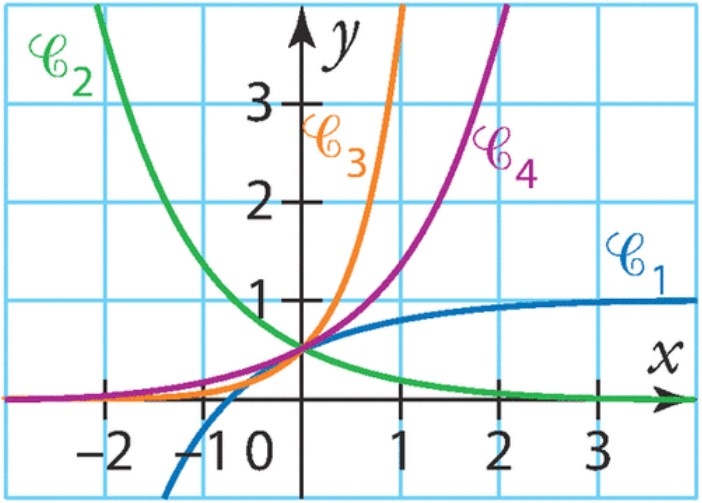
\includegraphics[width=5cm]{courbes1.jpg}}

\exo{}
On a représenté ci-dessous les courbes de certaines solutions de l'équation différentielle $y'=\dfrac{1}{2}y$.\\
On considère dans les questions suivantes toutes les solutions de l'équation.\\[.5em]
\dleft{10.5cm}{
    \begin{enumerate}
        \item Soit un point $M_0$ de coordonnées $(x_0\ ;y_0)$.\\
        Combien de courbes passent par le point $M_0$ ?
        \item Montrer que les tangentes à toutes les courbes au point d'ordonnée $2$ sont parallèles à la droite d'équation $y=x$.
    \end{enumerate}
}
{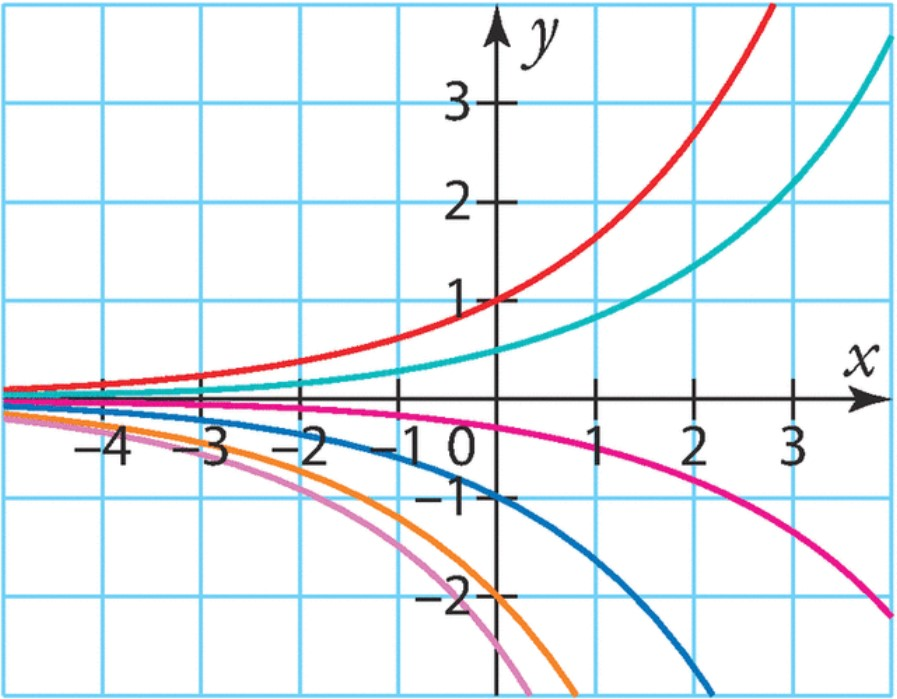
\includegraphics[width=6cm]{courbes2.jpg}}

\exo{}
\dleft{11.5cm}{
    Une note de musique est émise en pinçant la corde d'une guitare électrique.    La puissance du son émis, initialement de 100 watts, diminue avec le temps $t$, mesuré en secondes.\\
    On modélise par $f(t)$ la puissance du son émis, exprimée en watts, $t$ secondes après le pincement de la corde. Le son s'affaiblit à une vitesse proportionnelle à sa puissance, il a été établi que le coefficient de proportionnalité est $-0,12$.
}
{
\includegraphics[width=5cm]{guitare.jpg}}
\begin{enumerate}
    \item \faInfo \hspace*{0.1cm} \textit{Si $f$ est la fonction puissance, alors la vitesse d'évolution de cette puissance est $f'$.}\\
    Écrire l'équation différentielle traduisant la diminution de la puissance du son émis.
    \item Déterminer la fonction $f$ solution de cette équation différentielle qui vérifie la condition initiale $f(0)=100$.
    \item Quelle est la puissance du son émis deux secondes après le pincement de la corde ?
    \item Résoudre par le calcul l'équation $f(t)=80$, on donnera la valeur exacte et une valeur approchée à $10^{-3}$ près. Interpréter ce résultat.
\end{enumerate}

\exo{}
\dleft{11.5cm}{
    Une fibre optique est un fil très fin en verre ou en plastique, qui a la propriété de conduire la lumière et sert dans la transmission d'un signal véhiculant des données. La puissance du signal, exprimée en milliwatts (mW), s'atténue au cours de la propagation, exprimée en km.
}
{
\includegraphics[width=5cm]{fiber-optic-2749588_1280.jpg}}
\vspace*{.2cm}

On admet que la fonction puissance $g$ est définie et dérivable sur $\fio{0}{+\infty}$ et qu'elle est solution sur cet intervalle de l'équation différentielle $y'+0,035y=0$.

\begin{enumerate}
    \item Résoudre l'équation différentielle $y'+0,035y=0$.
    \item Sachant que $g(0)=7$, déterminer $g(x)$.
    \item Pour rester détectable, un signal doit être amplifié dès que sa puissance devient inférieure à $0,08$ mW.\\
    Le signal sera-t-il encore detecté au bout de 100 km de propagation ?
\end{enumerate}

\subsection*{Résoudre une équation différentielle de la forme $y'=ay+b$}

\exo{}
Choisir la bonne réponse :
\begin{enumerate}
    \item Une solution particulière de l'équation différentielle $y'+\dfrac{1}{2}y=10$ est :
    \begin{multicols}{4}
        \begin{enumerate}[label=\ding{111}]
            \item $20$
            \item $-20$
            \item $10$
            \item $-10$
        \end{enumerate}
    \end{multicols}

    \item Une solution de l'équation différentielle $y'=2y+2$ est :
    \begin{multicols}{4}
        \begin{enumerate}[label=\ding{111}]
            \item $f:x\mapsto e^{-2x}+1$
            \item $g:x\mapsto e^{-2x}-1$
            \item $h:x\mapsto e^{2x}+1$
            \item $k:x\mapsto e^{2x}-1$
        \end{enumerate}
    \end{multicols}

    \item La fonction $f$ définie sur $\R$ par $f(x)=2-e^{-4x}$ est solution de l'équation différentielle :
    \begin{multicols}{2}
        \begin{enumerate}[label=\ding{111}]
            \item $y'-4y=8$
            \item $y'-2y=8$
            \item $y'-8y=4$
            \item $y'+4y=8$
        \end{enumerate}
    \end{multicols}
\end{enumerate}

\exo{}
Résoudre les équations différentielles suivantes :
\begin{multicols}{2}
    \begin{enumerate}
        \item $y'=2y-1$
        \item $y'+2y=3$
    \end{enumerate}
\end{multicols}

\exo{}
\begin{enumerate}
    \item Résoudre $y'-2y=5$.
    \item Déterminer la solution $f$ de cette équation différentielle telle que $f(0)=0$.
\end{enumerate}

\exo{}
On considère l'équation différentielle $(E) : y'-5y=3$.
\begin{enumerate}
    \item Résoudre l'équation différentielle $(E)$.
    \item Déterminer la solution $f$ de $(E)$ telle que $f(0)=\dfrac{-6}{5}$.
    \item Étudier les variations de la fonction $f$ sur $\R$.
    \item Déterminer les limites de $f$ en $+\infty$ et $-\infty$.
    \item Déterminer la valeur de $x$ pour laquelle $f(x)=-10$.
\end{enumerate}

\exo{ Décharge d'un condensateur physique}
\dleft{12cm}{
    Un condensateur de capacité $C$ farads est chargé sous une tension initiale de 20 volts. Il se décharge ensuite dans une résistance de $R$ ohms.\\
    En notant $u(t)$ la tension (en volts) aux bornes du condensateur au bout de $t$ secondes, $u$ est alors une fonction définie sur $\fio{0}{+\infty}$ qui est solution de l'équation différentielle $y'+\dfrac{1}{RC}y=0$.
}
{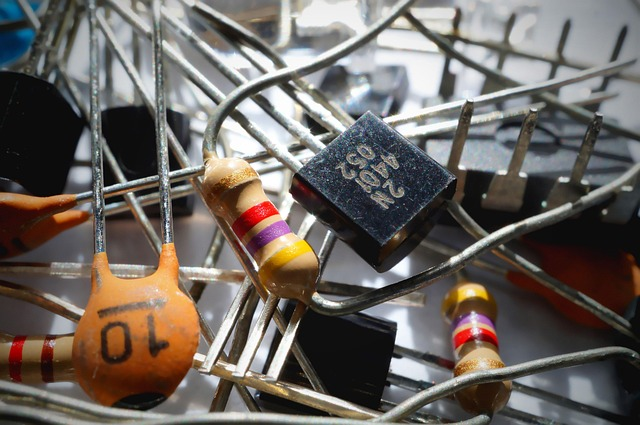
\includegraphics[width=4.5cm]{capacitor-1835729_640.jpg}}
\begin{enumerate}
    \item Résoudre l'équation différentielle $y'+\dfrac{1}{RC}y=0$ et en déduire l'expression de la fonction $u$.
    \item On suppose que $R=1000$ et $C=10^{-4}$.\\
    Pendant combien de temps (au centième de seconde près) la tension aux bornes du condensateur reste-t-elle supérieure ou égale à 5 volts ?
\end{enumerate}

\exo{ Loi de refroidissement de Newton}
Un corps est placé dans une enceinte dont on maintient la température constante égale à 20°C. À l'instant initial $t=0$, la température du corps est de 70°C et, après 5 min, elle n'est plus que de 60°C.\\
La température du corps en fonction du temps (en min) est notée $T(t)$. $T$ est une fonction définie sur $\fio{0}{+\infty}$. La loi de refroidissement de Newton énonce que $T'$ est propotionnelle à $T-20$.
\begin{enumerate}
    \item Justifier que la fonction $t\mapsto T(t)-20$ est solution d'une équation différentielle de la forme $y'=ay$, puis déterminer la fonction $T$.
    \item Déterminer la température du corps (au degré près) après une demi-heure.
    \item Après combien de temps (à la minute près) la température du corps sera-t-elle de 40°C ?
\end{enumerate}

\newpage
\exo{ Croissance de bactéries}
La nombre de bactéries $B$ d'une culture passe de 600 à l'instant initial à 1800 après 2 heures. On suppose que le taux de croissance est directement proportionnel au nombre de bactéries présentes.\\[.5em]
Déterminer :
\begin{enumerate}
        \item Une équation avec des conditions qui traduisent le problème.
        \item Une formule qui permet de calculer le nombre de bactéries $B(t)$ à l'instant $t$.
        \item Le nombre de bactéries après 4 heures.
        \item Le temps nécessaire pour que le nombre de bactéries dépasse 12 000.
\end{enumerate}

\exo{ En économie}
Dans une économie keynésienne simple, la consommation $C$ s'exprime par l'égalité $C=360+0,8Y$ et $I=120$, où $Y$ est le revenu et $I$ l'investissement.\\
Lorsque le marché est hors de l'équilibre, on suppose que le revenu $Y$ évolue en fonction du temps selon l'équation différentielle $Y'=0,25(C+I-Y)$.\\
À la période initiale, le revenu $Y_0$ est égal à 2000.
\begin{enumerate}
    \item Écrire l'équation différentielle vérfiée par la fonction $Y$.
    \item Déterminer la fonction $Y$.
    \item Étudier la limite de la fonction $Y$ en $+\infty$ et en déduire une conclusion sur la stabilité de l'équilibre de cette économie.
\end{enumerate}
\end{document}